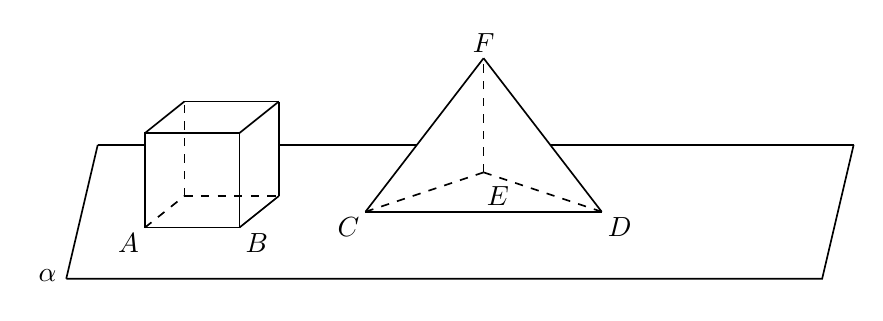
\begin{tikzpicture}[x=1cm,y=1cm,font=\normalsize,
  edge/.style={draw=black,solid,line width=.6pt},
  hide/.style={draw=black,dashed,line width=.6pt}]
% Ground plane alpha with cube (left) and tetrahedron (right)
\coordinate (P1) at (-3.2,-1.2);
\coordinate (P2) at (6.4,-1.2);
\coordinate (P3) at (6.8000000000,0.5000000000);
\coordinate (P4) at (-2.8000000000,0.5000000000);
\draw[edge] (P1)--(P2)--(P3);\draw[edge] (P4)--(P1);
\draw[edge] (P4)--(-2.2,.5) (-.5,.5)--(1.2538461538,.5) (2.9461538462,.5)--(P3);
% cube front face
\coordinate (A) at (-2.2,-0.55);
\coordinate (B) at (-1.0,-0.55);
\coordinate (A2) at (-2.2,0.65);
\coordinate (B2) at (-1.0,0.65);
\coordinate (A3) at (-1.7,1.05);
\coordinate (B3) at (-0.5,1.05);
\draw[edge] (A)--(B)--(B2)--(A2)--cycle;
\draw[edge] (A2)--(A3);
\draw[edge] (B2)--(B3);
\draw[edge] (A3)--(B3);
\draw[hide] (A)--(-1.7,-0.15);
\draw[edge] (B)--(-0.5000000000,-0.1500000000);
\draw[edge] (-0.5000000000,-0.1500000000)--(B3);
\draw[hide] (-1.7,-0.15)--(-0.5,-0.15);
\draw[hide] (-1.7,-0.15)--(-1.7,1.05);
% tetrahedron
\coordinate (C) at (0.6,-0.35);
\coordinate (Dd) at (3.6,-0.35);
\coordinate (E) at (2.1,0.15);
\coordinate (F) at (2.1,1.6);
\draw[edge] (C)--(Dd);
\draw[edge] (C)--(F);
\draw[edge] (Dd)--(F);
\draw[hide] (C)--(E);
\draw[hide] (Dd)--(E);
\draw[hide] (E)--(F);
\node[below left,inner sep=2pt] at (A) {$A$};
\node[below right,inner sep=2pt] at (B) {$B$};
\node[below left,inner sep=2pt] at (C) {$C$};
\node[below right,inner sep=2pt] at (Dd) {$D$};
\node[below right,inner sep=2pt,xshift=-1pt,yshift=-3pt] at (E) {$E$};
\node[above,inner sep=2pt] at (F) {$F$};
\node[below left,inner sep=4pt,xshift=-5pt,yshift=-1pt] at (-3.0,-0.9) {$\alpha$};
\end{tikzpicture}
